%% ----------------------------------------------------------------------------
%%  §9.7  Calcolo di aree e altre applicazioni
%% ----------------------------------------------------------------------------
\needspace{10\baselineskip}
\section{Calcolo di aree e altre applicazioni}
\label{sec:applicazioni-integrali}

\subsection{Aree di figure piane}

Abbiamo introdotto l'integrale definito con lo scopo principale di calcolare aree di
figure piane del tipo $A=\set{(x,y) \tc a\le x\le b,\ 0\le y\le f(x)}$, con $f$ continua e non
negativa in $[a,b]$; in tal caso l'area di $A$ è $\int_{a}^{b}f(x)\,dx$
\eqref{eq:area-rettangoloide}. Più in generale consideriamo una regione delimitata dai
grafici di due funzioni continue $f$, $g$ con $g\le f$ in $[a,b]$ (\cref{fig:area-tra-curve}):
\begin{equation}\label{eq:regione-normale}
  T=\set{(x,y)\in\R^{2} \tc a\le x\le b,\ g(x)\le y\le f(x)} .
\end{equation}
Se $g\ge0$, la regione $T$ si ottiene togliendo dal rettangoloide di $f$ quello di $g$
(tranne i punti del grafico di $g$, che non hanno area), e la sua area è la differenza
delle due aree. Se $g$ assume anche valori negativi, si trasla tutto verso l'alto di una
costante $k$ tale che $g+k\ge0$: la traslazione non cambia le aree, e
$\int_{a}^{b}(f+k)-\int_{a}^{b}(g+k)=\int_{a}^{b}(f-g)$. In ogni caso, dunque,
\begin{equation}\label{eq:area-tra-curve}
  \text{area di }T=\int_{a}^{b}\bigl[f(x)-g(x)\bigr]\,dx ,
\end{equation}
formula che prendiamo come definizione dell'area di una regione del tipo
\eqref{eq:regione-normale}.

\begin{figure}[htb]
\centering
\begin{tikzpicture}
\begin{axis}[name=r1, width=0.52\textwidth, height=4.8cm, axis lines=left, axis on top, xmin=0,
  xmax=4.6, ymin=0, ymax=3.2, xtick={0.7,4.0}, xticklabels={$a$,$b$}, ytick=\empty,
  title={\scriptsize la regione $T$}]
  \addplot[draw=none, fill=blu!22, domain=0.7:4.0, samples=50]
    {2.3+0.3*sin(deg(1.5*x))} \closedcycle;
  \addplot[draw=none, fill=white, domain=0.7:4.0, samples=50]
    {1.0+0.25*cos(deg(1.2*x))} \closedcycle;
  \addplot[curva, domain=0.5:4.2, samples=80] {2.3+0.3*sin(deg(1.5*x))};
  \addplot[curva2, domain=0.5:4.2, samples=80] {1.0+0.25*cos(deg(1.2*x))};
  \addplot[tratteggio] coordinates {(0.7,0) (0.7,2.560)};
  \addplot[tratteggio] coordinates {(4.0,0) (4.0,2.216)};
  \node[font=\scriptsize, blu] at (axis cs:2.3,1.7) {$T$};
  \node[font=\scriptsize, anchor=south] at (axis cs:2.7,2.62) {$y=f(x)$};
  \node[font=\scriptsize, rame, anchor=north] at (axis cs:2.2,0.72) {$y=g(x)$};
\end{axis}
\begin{axis}[at={(r1.east)}, anchor=west, xshift=0.7cm, width=0.46\textwidth,
  height=4.8cm, axis lines=middle, xmin=-1.4, xmax=1.5, ymin=-0.15, ymax=1.35,
  xtick={-1,1}, ytick={1}, yticklabel style={anchor=south east, font=\scriptsize},
  title={\scriptsize segmento parabolico: area $\frac43$}]
  \addplot[draw=none, fill=blu!22, domain=-1:1, samples=50] {x^2} -- (axis cs:1,1)
    -- (axis cs:-1,1) -- cycle;
  \addplot[curva, domain=-1.2:1.2, samples=60] {x^2};
  \addplot[curva2, domain=-1.3:1.3] {1};
  \draw[grigio, densely dashed] (axis cs:-1,1) -- (axis cs:0,0) -- (axis cs:1,1);
\end{axis}
\end{tikzpicture}
\caption{A sinistra, una regione delimitata dai grafici di due funzioni: la sua area è
$\int_{a}^{b}(f-g)$. A destra, il segmento parabolico tra $y=x^{2}$ e la corda $y=1$: la sua
area è i $\frac43$ di quella del triangolo inscritto (tratteggiato), come aveva scoperto
Archimede.}
\label{fig:area-tra-curve}
\end{figure}

Ad esempio, il segmento parabolico compreso tra la parabola $y=x^{2}$ e la retta $y=1$ ha
area $\int_{-1}^{1}(1-x^{2})\,dx=\bigl[x-\frac{x^{3}}3\bigr]_{-1}^{1}=\frac43$, mentre il triangolo
inscritto di vertici $(\pm1,1)$ e $(0,0)$ ha area $1$: ritroviamo il rapporto $\frac43$ di
Archimede (\cref{fig:area-tra-curve}, a destra).

\needspace{9\baselineskip}
\begin{esempio}[Area del cerchio e dell'ellisse]\label{es:cerchio-ellisse}
Il cerchio di centro l'origine e raggio $r$ è la regione
\[
  C=\set{(x,y)\in\R^{2} \tc -r\le x\le r,\ -\sqrt{r^{2}-x^{2}}\le y\le\sqrt{r^{2}-x^{2}}} ,
\]
del tipo \eqref{eq:regione-normale}. Per la \eqref{eq:area-tra-curve} e la sostituzione $x=rt$
(\cref{teo:sostituzione-definita}), e poi per la \eqref{eq:area-semicerchio},
\begin{equation}\label{eq:area-cerchio-integrale}
\begin{split}
  \text{area di }C&=2\int_{-r}^{r}\sqrt{r^{2}-x^{2}}\,dx
  =2\int_{-1}^{1}\sqrt{r^{2}-r^{2}t^{2}}\,r\,dt\\
  &=2r^{2}\int_{-1}^{1}\sqrt{1-t^{2}}\,dt=\pi r^{2} .
\end{split}
\end{equation}
La regione racchiusa dall'ellisse $\frac{x^{2}}{a^{2}}+\frac{y^{2}}{b^{2}}=1$ ($a,b>0$) è
\[
  E=\Bigl\{(x,y)\in\R^{2} \tc -a\le x\le a,\ \abs y\le\frac ba\sqrt{a^{2}-x^{2}}\Bigr\} ,
\]
e con la sostituzione $x=at$
\begin{equation}\label{eq:area-ellisse}
\begin{split}
  \text{area di }E&=2\,\frac ba\int_{-a}^{a}\sqrt{a^{2}-x^{2}}\,dx\\
  &=2ab\int_{-1}^{1}\sqrt{1-t^{2}}\,dt=\pi ab .
\end{split}
\end{equation}
Per un'ala di pianta ellittica con apertura $b$ e corda alla radice $c_{0}$ (i semiassi
sono $\frac b2$ e $\frac{c_{0}}2$) la superficie alare è quindi $S=\frac\pi4\,c_{0}b$, e
l'allungamento è $AR=\frac{b^{2}}S=\frac{4b}{\pi c_{0}}$: per un'ala come quella della
\cref{fig:portanza-ellittica}, con $b=10$~m e $c_{0}=1{,}6$~m, $S\approx12{,}57$~m$^{2}$ e
$AR\approx7{,}96$.
\end{esempio}

\subsection{Il tempo di salita}

\begin{esempio}[Tempo di salita e quota di tangenza]\label{es:tempo-salita}
Per un velivolo con motore a pistoni aspirato la velocità di salita massima diminuisce
con la quota, in prima approssimazione linearmente:
\[
  v_{z}(h)=v_{z0}\Bigl(1-\frac hH\Bigr), \qquad 0\le h<H ,
\]
dove $H$ è la \emph{quota di tangenza teorica}, alla quale il velivolo non riesce più a
salire. Se $h(t)$ è la quota all'istante $t$, salendo sempre alla massima velocità di
salita si ha $h'(t)=v_{z}(h(t))>0$; la funzione $h(t)$ è strettamente crescente, e la sua
inversa $t(h)$, il tempo necessario per raggiungere la quota $h$, ha derivata
$t'(h)=\frac1{v_{z}(h)}$ (\cref{teo:derivata-inversa}). Per la formula fondamentale e la
\eqref{eq:argomento-lineare},
\begin{equation}\label{eq:tempo-salita}
  t(h)=\int_{0}^{h}\frac{d\eta}{v_{z0}(1-\eta/H)}
  =\Bigl[-\frac H{v_{z0}}\log\Bigl(1-\frac\eta H\Bigr)\Bigr]_{0}^{h}
  =\frac H{v_{z0}}\log\frac H{H-h} .
\end{equation}
Con $v_{z0}=5$~m/s e $H=4000$~m, il tempo per salire a $3000$~m è
$800\log4\approx1109$~s, circa $18{,}5$ minuti. La \emph{quota di tangenza pratica} è
convenzionalmente quella alla quale la velocità di salita si riduce a $0{,}5$~m/s (circa
$100$ piedi al minuto): qui $h=0{,}9\,H=3600$~m, raggiunta in $800\log10\approx1842$~s,
circa $31$ minuti. Per $h\to H$ il tempo tende a $+\infty$: la quota di tangenza teorica non
si raggiunge in un tempo finito. Nel linguaggio del \cref{sec:impropri}, l'integrale
improprio $\int_{0}^{H}\frac{d\eta}{v_{z}(\eta)}$ è divergente.
\end{esempio}

\subsection{La pressione nella troposfera standard}

\begin{esempio}[La legge della pressione nell'atmosfera standard]\label{es:pressione-isa}
In un'atmosfera in quiete la pressione $p(h)$ diminuisce con la quota secondo la legge
dell'idrostatica $p'(h)=-\rho(h)\,g$, con $g=9{,}80665$~m/s$^{2}$, e l'aria segue l'equazione di stato dei gas
$p=\rho RT$, con $R=287{,}05$~J/(kg\,K). Nella troposfera dell'atmosfera standard la
temperatura decresce linearmente, $T(h)=T_{0}-Lh$, con $T_{0}=288{,}15$~K e
$L=0{,}0065$~K/m. Eliminando $\rho$,
\[
  \frac{d}{dh}\log p(h)=\frac{p'(h)}{p(h)}=-\frac g{R\,(T_{0}-Lh)} .
\]
Per la formula fondamentale applicata alla funzione $\log p$, e per la
\eqref{eq:argomento-lineare},
\[
\begin{aligned}
  \log\frac{p(h)}{p_{0}}&=-\frac gR\int_{0}^{h}\frac{d\eta}{T_{0}-L\eta}
  =\frac g{RL}\Bigl[\log(T_{0}-L\eta)\Bigr]_{0}^{h}\\
  &=\frac g{RL}\log\Bigl(1-\frac{Lh}{T_{0}}\Bigr),
\end{aligned}
\]
cioè
\begin{equation}\label{eq:pressione-isa}
  p(h)=p_{0}\Bigl(1-\frac{Lh}{T_{0}}\Bigr)^{g/(RL)}, \qquad \frac g{RL}\approx5{,}2559 .
\end{equation}
Con $p_{0}=101\,325$~Pa, alla tropopausa ($h=11\,000$~m, $T=216{,}65$~K) si ottiene
$p\approx22\,632$~Pa, il valore tabulato. Dividendo per $RT(h)$ si ottiene la densità
$\rho(h)=\rho_{0}\bigl(1-\frac{Lh}{T_{0}}\bigr)^{n}$ con $n=\frac g{RL}-1\approx4{,}2559$: è la formula
che nel \cref{cap:derivate} avevamo preso come dato per derivarla, e che qui abbiamo
\emph{ricavato} integrando.
\end{esempio}

\subsection{Taglio e momento flettente in un'ala}

Concludiamo con un'applicazione centrale delle costruzioni aeronautiche. In volo, la
semiala si comporta come una trave incastrata alla fusoliera (la radice, $y=0$) e libera
all'estremità ($y=s=\frac b2$), caricata dalla portanza distribuita $l(y)$. Trascuriamo il
peso proprio dell'ala. In ogni stazione $y$ la parte di semiala esterna, cioè
$[y,s]$, trasmette alla parte interna una forza, il \emph{taglio} $T(y)$, e un momento, il
\emph{momento flettente} $M(y)$, che equilibrano i carichi che agiscono su di essa. La
striscia $[\eta,\eta+d\eta]$ porta la forza $l(\eta)\,d\eta$, con braccio $\eta-y$ rispetto alla
stazione $y$; sommando,
\begin{equation}\label{eq:taglio-momento}
  T(y)=\int_{y}^{s}l(\eta)\,d\eta, \qquad M(y)=\int_{y}^{s}(\eta-y)\,l(\eta)\,d\eta .
\end{equation}

\begin{proposizione}[Relazioni tra carico, taglio e momento]\label{prop:taglio-momento}
Sia $l$ continua in $[0,s]$ e siano $T$, $M$ definiti dalle \eqref{eq:taglio-momento}.
Allora $T$ e $M$ sono derivabili, con
\begin{equation}\label{eq:relazioni-trave}
  T'(y)=-l(y), \qquad M'(y)=-T(y), \qquad T(s)=M(s)=0 ,
\end{equation}
e il momento alla radice vale
\begin{equation}\label{eq:momento-radice}
  M(0)=\int_{0}^{s}T(y)\,dy=\int_{0}^{s}y\,l(y)\,dy .
\end{equation}
\end{proposizione}

\begin{schema}
\Ipotesi{$l$ continua in $[0,s]$; \ $T$, $M$ come nelle \eqref{eq:taglio-momento}.}
\Tesi{$T'=-l$, $M'=-T$, $T(s)=M(s)=0$; \ $M(0)=\int_{0}^{s}T=\int_{0}^{s}yl$.}
\end{schema}

\begin{strategia}
Il taglio è una funzione integrale con estremo inferiore variabile, e il
\cref{cor:estremi-variabili} ne dà la derivata. Per il momento, la variabile $y$ compare
anche dentro l'integrale: la si porta fuori spezzando $\eta-y$, e si deriva un prodotto.
La seconda uguaglianza della \eqref{eq:momento-radice} è un'integrazione per parti.
\end{strategia}

\begin{dimostrazione}
Per il \cref{cor:estremi-variabili}, $T'(y)=-l(y)$; ovviamente $T(s)=M(s)=0$. Per la
linearità, $M(y)=\int_{y}^{s}\eta\,l(\eta)\,d\eta-y\,T(y)$; il primo addendo ha derivata
$-y\,l(y)$, ancora per il \cref{cor:estremi-variabili}, mentre il prodotto $y\,T(y)$, per la
regola di derivazione del prodotto, ha derivata $T(y)+y\,T'(y)=T(y)-y\,l(y)$. Dunque
$M'(y)=-y\,l(y)-T(y)+y\,l(y)=-T(y)$. Per la formula fondamentale,
$M(0)=M(0)-M(s)=-\int_{0}^{s}M'(y)\,dy=\int_{0}^{s}T(y)\,dy$. Infine, integrando per parti
(\cref{teo:per-parti-definito}) con fattore finito $T$ e fattore differenziale $1$,
\[
  \int_{0}^{s}T(y)\,dy=\Bigl[y\,T(y)\Bigr]_{0}^{s}-\int_{0}^{s}y\,T'(y)\,dy=0+\int_{0}^{s}y\,l(y)\,dy ,
\]
perché $T(s)=0$. (Il risultato si legge anche direttamente nella seconda delle
\eqref{eq:taglio-momento} con $y=0$.)
\end{dimostrazione}

\begin{esempio}[Taglio e momento per la distribuzione ellittica]\label{es:taglio-ellittico}
Per la distribuzione ellittica \eqref{eq:portanza-ellittica}, $l(y)=l_{0}\sqrt{1-(y/s)^{2}}$,
posto $u=\frac ys$, la sostituzione $\eta=sw$ e la \eqref{eq:integrale-semicerchio} danno
\begin{equation}\label{eq:taglio-ellittico}
  T(y)=l_{0}s\int_{u}^{1}\sqrt{1-w^{2}}\,dw
  =\frac{l_{0}s}2\Bigl[\frac\pi2-\arcsen u-u\sqrt{1-u^{2}}\Bigr] .
\end{equation}
Alla radice $T(0)=\frac\pi4\,l_{0}s=\frac W2$: ciascuna semiala trasmette alla fusoliera metà
del peso. Per il momento alla radice, la \eqref{eq:momento-radice} e la sostituzione
$w=1-(y/s)^{2}$, con $dw=-\frac{2y}{s^{2}}\,dy$, danno
\begin{equation}\label{eq:momento-ellittico}
  M(0)=l_{0}\int_{0}^{s}y\sqrt{1-\frac{y^{2}}{s^{2}}}\,dy=\frac{l_{0}s^{2}}2\int_{0}^{1}\sqrt w\,dw
  =\frac{l_{0}s^{2}}3=\frac{Wb}{3\pi} ,
\end{equation}
avendo usato $l_{0}=\frac{4W}{\pi b}$ e $s=\frac b2$. Il braccio della risultante $\frac W2$ è
$\frac{M(0)}{T(0)}=\frac{2b}{3\pi}=\frac{4s}{3\pi}$, l'ascissa del baricentro di un quarto di ellisse.
Per $W=10\,000$~N e $b=10$~m: $T(0)=5000$~N, $M(0)\approx10\,610$~N\,m, con un braccio di
circa $2{,}12$~m. Con un carico uniforme $l=\frac Wb$ il braccio sarebbe $\frac s2=2{,}5$~m e il
momento $\frac{Wb}8=12\,500$~N\,m: la distribuzione ellittica, concentrando la portanza verso
la radice, riduce il momento flettente alla radice di circa il $15\%$ (il rapporto è
$\frac8{3\pi}\approx0{,}849$).
\end{esempio}

\begin{figure}[htb]
\centering
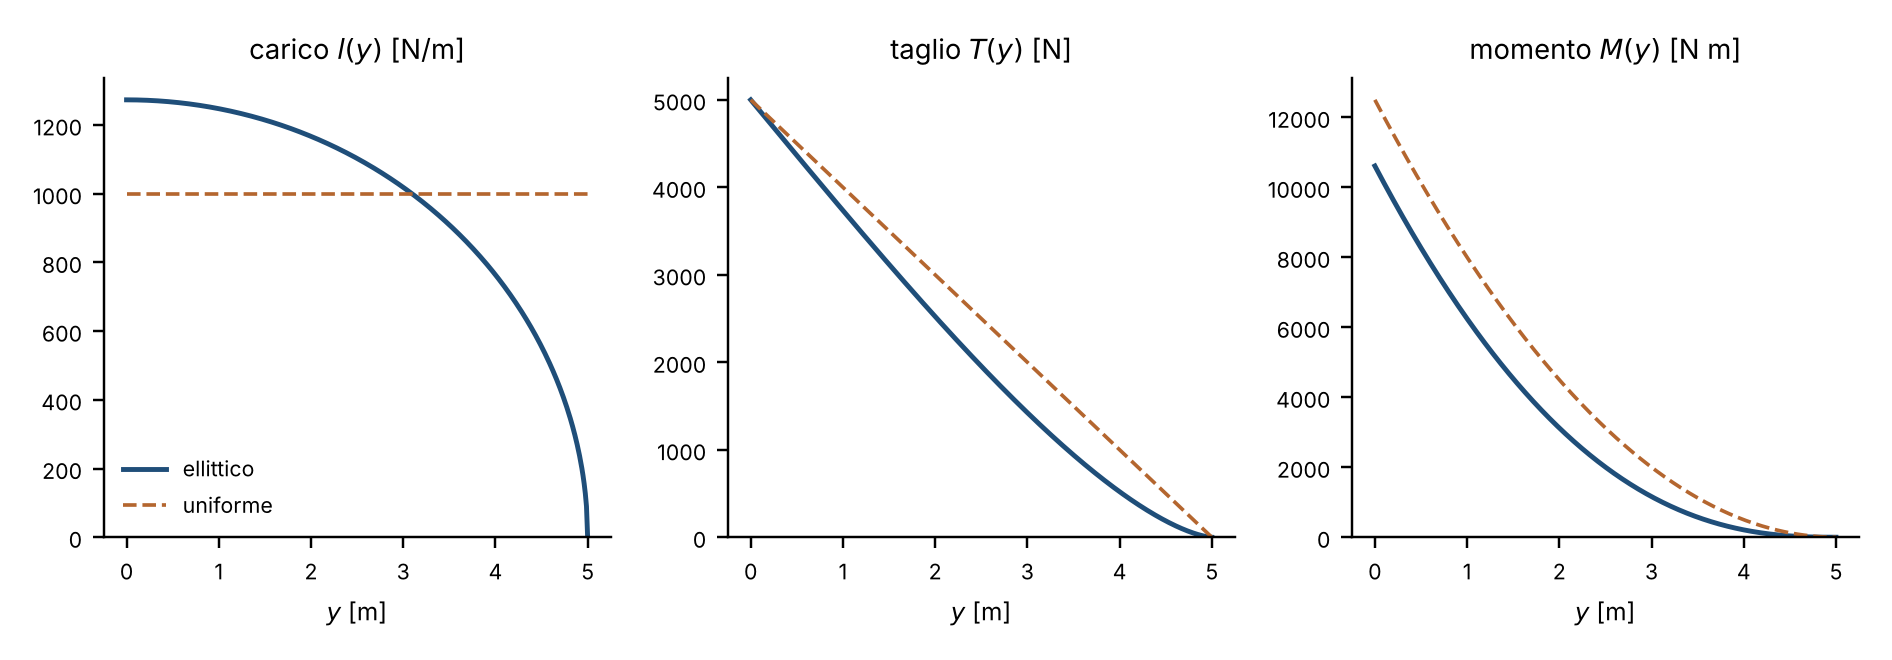
\includegraphics[width=\textwidth]{figure/taglio_momento.png}
\caption{Carico, taglio e momento flettente lungo la semiala per la distribuzione
ellittica ($W=10\,000$~N, $b=10$~m), confrontati con quelli di un carico uniforme con la
stessa portanza totale (tratteggio). Il taglio è l'area del carico all'esterno della
stazione, il momento l'area del taglio; le pendenze sono $T'=-l$ e $M'=-T$
(\texttt{python/fig\_taglio\_momento.py}).}
\label{fig:taglio-momento}
\end{figure}

Il programma seguente calcola il taglio e il momento numericamente, integrando il
carico dall'estremità verso la radice con la formula dei trapezi, e li confronta con le
formule \eqref{eq:taglio-ellittico} e \eqref{eq:momento-ellittico}.

\begin{python}[Taglio e momento flettente lungo la semiala]
import math

W, b = 10000.0, 10.0
s, l0 = b / 2, 4 * W / (math.pi * b)
l = lambda y: l0 * math.sqrt(max(0.0, 1 - (y / s)**2))

def T_esatto(y):
    u = y / s
    q = math.pi / 2 - math.asin(u) - u * math.sqrt(1 - u * u)
    return l0 * s / 2 * q

n = 5000                     # trapezi, dall'estremità alla radice
h = s / n
y = [s - k * h for k in range(n + 1)]
T, M = [0.0], [0.0]
for k in range(1, n + 1):
    T.append(T[-1] + h * (l(y[k - 1]) + l(y[k])) / 2)    # T' = -l
    M.append(M[-1] + h * (T[k - 1] + T[k]) / 2)          # M' = -T
print("  y [m]   T num. [N]  T esatto [N]   M num. [N m]")
for k in range(n, -1, -1000):
    print(f"{y[k]:6.1f}  {T[k]:10.1f}  {T_esatto(y[k]):11.1f}"
          f"  {M[k]:12.1f}")
print(f"M(0) esatto = W b/(3 pi) = {W * b / (3 * math.pi):.1f} N m")
\end{python}
\begin{risultato}
  y [m]   T num. [N]  T esatto [N]   M num. [N m]
   0.0      5000.0       5000.0       10610.3
   1.0      3735.3       3735.3        6244.8
   2.0      2523.2       2523.2        3122.3
   3.0      1423.8       1423.8        1161.1
   4.0       520.4        520.4         210.1
   5.0         0.0          0.0           0.0
M(0) esatto = W b/(3 pi) = 10610.3 N m
\end{risultato}

\begin{osservazione}[Un carico concentrato: il motore in ala]\label{oss:motore-ala}
Supponiamo che la semiala porti, oltre alla portanza $l$, il peso $P$ di un motore,
applicato nella stazione $y_{m}\in(0,s)$ e diretto verso il basso. Per $y<y_{m}$ il tratto
esterno $[y,s]$ comprende il motore, e le \eqref{eq:taglio-momento} diventano
\[
\begin{aligned}
  T(y)&=\int_{y}^{s}l(\eta)\,d\eta-P,\\
  M(y)&=\int_{y}^{s}(\eta-y)\,l(\eta)\,d\eta-P\,(y_{m}-y) \qquad (0\le y<y_{m}),
\end{aligned}
\]
mentre per $y\ge y_{m}$ restano invariate. Il taglio ha in $y_{m}$ un salto $P$; il
momento è continuo, ma ha in $y_{m}$ un punto angoloso, e $M'=-T$ vale soltanto per
$y\neq y_{m}$ (con la dimostrazione della \cref{prop:taglio-momento}). Dunque $M$ è
continua e regolare a tratti, e per il \cref{teo:formula-regolari-tratti}
$M(0)=-\int_{0}^{s}M'\,dy=\int_{0}^{s}T\,dy$: il momento alla radice è ancora l'area del
diagramma del taglio, mentre la stessa formula applicata al taglio, discontinuo,
sbaglierebbe di $P$ (\cref{oss:regolari-tratti-salti}). Si ha poi
$M(0)=\int_{0}^{s}y\,l(y)\,dy-P\,y_{m}$: il motore \emph{riduce} il momento alla radice, ed
è uno dei motivi per cui motori e combustibile si sistemano in ala. Con i dati
dell'\cref{es:taglio-ellittico}, $P=1000$~N e $y_{m}=1{,}5$~m, il momento scende da circa
$10\,610$ a circa $9\,110$~N\,m.
\end{osservazione}

\begin{notastorica}[Dalla trave di Galileo alle ali a sbalzo]
Il problema della resistenza di una trave incastrata a un estremo e caricata, la
\emph{mensola} o trave a sbalzo, fu posto da Galileo nei \emph{Discorsi e dimostrazioni
matematiche intorno a due nuove scienze} (1638), che lo risolse in modo errato quanto
alla distribuzione delle tensioni nella sezione. Le relazioni differenziali
$T'=-l$, $M'=-T$ e la teoria della flessione si consolidarono nel Settecento e
nell'Ottocento, con Jakob Bernoulli, Eulero e Navier. Tra le prime ali a sbalzo di impiego pratico, prive di
montanti e tiranti esterni, vi furono quelle realizzate da Hugo Junkers nel 1915 con il monoplano
metallico J~1: da allora il calcolo del taglio e del momento flettente lungo l'apertura,
cioè l'integrazione ripetuta della distribuzione di portanza, è il punto di partenza del
dimensionamento strutturale di ogni ala.
\end{notastorica}
